\section{奇异同调}
\label{sec:homol-singular-homology}

单纯同调的输入是一个复形。圆周、环带这样的空间本身并没有指定三角剖分；同一个空间可以有许多不同的三角剖分，单纯同调是否与选择无关，从定义上看不出来。环带与圆周同伦等价，它们的同调是否相同，也无法在两个毫不相干的复形之间直接比较。

解决的办法是不再要求单纯形是复形中规定好的一块，而允许它是标准单纯形到空间的任意连续映射。这样就不用选择三角剖分，同调直接定义在拓扑空间上。代价是链空间变得极大，无法直接求秩。下面先给出构造及连续映射诱导的同调映射，再说明它在有限复形上与单纯同调一致，最后证明同伦不变性。

\subsection{奇异同调的构造}
\label{sec:homol-singular-construction}

在复形中，一条有向边是从一个顶点到另一个顶点的线段。在一般空间中，对应的对象应当是一条路径，即$\Delta^1\cong[0,1]$到空间的连续映射。三角形对应$\Delta^2$到空间的连续映射，它可以被压扁、折叠，甚至退化成一点。

\begin{definition}[奇异单形与奇异链]
\label{def:homol-singular-simplex}
设$X$为拓扑空间。连续映射$\sigma:\Delta^k\to X$称为$X$中的$k$维\term{奇异单形}（singular simplex）。以全部$k$维奇异单形为基的实向量空间记为$S_k(X)$，其元素是奇异单形的有限线性组合，称为$k$维奇异链；$k<0$时$S_k(X)=0$。
\end{definition}

\begin{BookInlineFigure}
  \centering
  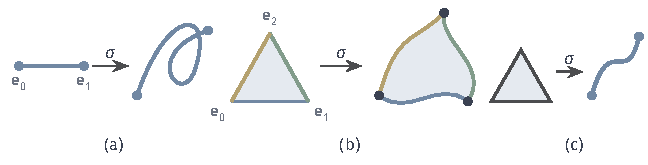
\includegraphics[width=109.657mm]{figures/04-spaces-measures-and-geometry/01-topology-and-metric/tikz/homol-singular-simplices/figure.pdf}
  \caption{奇异单形是连续映射，其像可以弯曲或退化。(a)$\sigma:\Delta^1\to X$是一条路径，允许自相交。(b)$\sigma:\Delta^2\to X$，蓝、绿、黄三条边是三个面$\sigma\circ\delta_2,\sigma\circ\delta_0,\sigma\circ\delta_1$的像。(c)$\Delta^2$可以被整个压到一条曲线上，它仍是一个合法的二维奇异单形。}
  \label{fig:homol-singular-simplices}
\end{BookInlineFigure}

$S_k(X)$通常是无穷维的：$X$中的每个点都是一个$0$维奇异单形，每条路径都是一个$1$维奇异单形，如图~\ref{fig:homol-singular-simplices}所示。但每个奇异链只涉及有限个奇异单形，所以下面的线性代数操作都是有限的。

\paragraph{奇异边界}
在复形中，$k$-单纯形的第$i$个面是去掉第$i$个顶点。对奇异单形，把它限制到$\Delta^k$的第$i$个面上即可。先用下面的映射把低一维的标准单纯形放到这个面上，它在第$i$个位置插入零：
\[
 \delta_i:\Delta^{k-1}\to\Delta^k,\qquad
 \delta_i(t_0,\ldots,t_{k-1})=(t_0,\ldots,t_{i-1},0,t_i,\ldots,t_{k-1}).
\]

这个映射把$\Delta^{k-1}$线性地送到$\Delta^k$中与$\bm e_i$相对的面上，并保持其余顶点的次序。奇异单形的边界就定义为
\begin{equation}
 \partial_k\sigma=\sum_{i=0}^k(-1)^i\,\sigma\circ\delta_i,
 \label{eq:homol-singular-boundary}
\end{equation}
线性延拓到$S_k(X)$。每个$\sigma\circ\delta_i$都是连续映射的复合，是$(k-1)$维奇异单形。对路径$\sigma$，
\[
 \partial_1\sigma=\sigma\circ\delta_0-\sigma\circ\delta_1=\sigma(\bm e_1)-\sigma(\bm e_0),
\]
仍是终点减起点。

\begin{example}[平面上一个奇异三角形的边界]
\label{ex:homol-singular-boundary}
取$X=\mathbb R^2$与线性映射
\[
 \sigma(t_0,t_1,t_2)=(t_1,t_2).
\]
它把$\Delta^2$送到顶点为$(0,0),(1,0),(0,1)$的三角形上，$\bm e_0,\bm e_1,\bm e_2$依次对应这三点。三个面依次是
\begin{align*}
 (\sigma\circ\delta_0)(s_0,s_1)&=\sigma(0,s_0,s_1)=(s_0,s_1),\\
 (\sigma\circ\delta_1)(s_0,s_1)&=\sigma(s_0,0,s_1)=(0,s_1),\\
 (\sigma\circ\delta_2)(s_0,s_1)&=\sigma(s_0,s_1,0)=(s_1,0).
\end{align*}
它们分别是从$(1,0)$到$(0,1)$、从$(0,0)$到$(0,1)$、从$(0,0)$到$(1,0)$的线段。由式~\eqref{eq:homol-singular-boundary}，
\[
 \partial_2\sigma=\sigma\circ\delta_0-\sigma\circ\delta_1+\sigma\circ\delta_2,
\]
正负号使三段路径沿三角形绕行一周，与单纯情形的$\partial_2[v_0,v_1,v_2]$一致。
\end{example}

\begin{lemma}[奇异边界的边界为零]
\label{lem:homol-singular-boundary-squared}
对$i<j$，作为$\Delta^{k-2}\to\Delta^k$的映射，
\begin{equation}
 \delta_j\circ\delta_i=\delta_i\circ\delta_{j-1}.
 \label{eq:homol-face-identity}
\end{equation}
因此$\partial_{k-1}\circ\partial_k=0$。
\end{lemma}

\begin{proof}
式~\eqref{eq:homol-face-identity}的两边都在第$i$与第$j$个位置插入零，其余坐标依次排在剩下的位置上。左边先在第$i$位插零，再在第$j$位插零。右边先在第$j-1$位插零，再在更靠前的第$i$位插零，使前一个零后移到第$j$位。所以两边相同。

展开两次边界，得到
\[
 \partial\partial\sigma=\sum_{j=0}^k\sum_{i=0}^{k-1}(-1)^{i+j}\sigma\circ\delta_j\circ\delta_i.
\]
按$i<j$与$i\geq j$分成两组。第一组用式~\eqref{eq:homol-face-identity}改写，再令$j'=j-1\geq i$，得到
\[
 \sum_{i<j}(-1)^{i+j}\sigma\circ\delta_i\circ\delta_{j-1}
 =-\sum_{i\leq j'}(-1)^{i+j'}\sigma\circ\delta_i\circ\delta_{j'}.
\]
第二组把求和字母改写为$a=j\leq b=i$，得到
\[
 \sum_{a\leq b}(-1)^{a+b}\sigma\circ\delta_a\circ\delta_b.
\]
两组逐项相消。
\end{proof}

这与定理~\ref{thm:homol-boundary-squared}是同一个机制：去掉两个顶点的两种先后次序以相反的符号出现。于是$(S_k(X),\partial_k)$是链复形。

\begin{definition}[奇异同调]
\label{def:homol-singular-homology}
拓扑空间$X$的$k$维（实系数）\term{奇异同调}（singular homology）空间定义为
\begin{equation}
 H_k(X)=\ker\partial_k/\operatorname{im}\partial_{k+1}.
 \label{eq:homol-singular-homology}
\end{equation}
闭链、边界链与同调类的说法与单纯情形相同。
\end{definition}

\begin{BookInlineTable}
  \centering
  \caption{单纯同调与奇异同调}
  \label{tab:homol-simplicial-vs-singular}
  \begin{tabular}{lll}
    \toprule
    & 单纯同调 & 奇异同调 \\
    \midrule
    输入 & 有限复形 & 任意拓扑空间 \\
    $k$维基向量 & $k$-单纯形，有限个 & 连续映射$\Delta^k\to X$ \\
    取边界 & 去掉第$i$个顶点 & 限制到第$i$个面 \\
    可否直接求秩 & 可以 & 不可以，维数无穷 \\
    是否依赖选择 & 依赖复形 & 只依赖空间 \\
    \bottomrule
  \end{tabular}
\end{BookInlineTable}

表~\ref{tab:homol-simplicial-vs-singular}比较了两种构造。奇异同调的优点和缺点恰好与单纯同调互补，第~\ref{sec:homol-simplicial-singular}小节要把二者接起来。

\paragraph{零维同调与路径分支}
零维奇异单形就是$X$中的点，一维奇异单形就是路径，其边界是终点减起点。所以零维同调的计算与定理~\ref{thm:homol-h0-components}平行，只是图的路径换成了空间中的路径。

\begin{theorem}[零维奇异同调计数路径分支]
\label{thm:homol-singular-h0}
设$X$的路径分支为$\{P_\alpha\}$，从每个$P_\alpha$中取一点$x_\alpha$。则$\{[x_\alpha]\}$是$H_0(X)$的一组基；特别地，$X$非空且路径连通时，$H_0(X)\cong\mathbb R$。
\end{theorem}

\begin{proof}
若$x,y$在同一路径分支中，取从$y$到$x$的路径$\sigma$，则$x-y=\partial_1\sigma$，二者同调。所以$\{[x_\alpha]\}$张成$H_0(X)$。

对每个分支$P_\alpha$定义线性函数$\varphi_\alpha$：把$0$维链在$P_\alpha$中各点上的系数相加。路径$\sigma$的像是路径连通集，起点与终点同属一个路径分支，所以$\varphi_\alpha(\partial_1\sigma)=0$，$\varphi_\alpha$在边界链上为零，在$H_0(X)$上有定义。

若有限组合$\sum\lambda_\alpha[x_\alpha]=0$，用$\varphi_\beta$作用得$\lambda_\beta=0$，所以它们线性无关。
\end{proof}

\paragraph{连续映射诱导的同调映射}
奇异同调的好处在于，任何连续映射都能直接作用在链上：奇异单形与连续映射复合，仍是奇异单形。单纯同调做不到这一点，一个连续映射通常不把单纯形送到单纯形。

\begin{theorem}[连续映射诱导同调映射]
\label{thm:homol-induced-map}
设$f:X\to Y$连续。令$f_\#\sigma=f\circ\sigma$并线性延拓，则$f_\#:S_k(X)\to S_k(Y)$是链映射，诱导线性映射$f_*:H_k(X)\to H_k(Y)$。并且$(\operatorname{id}_X)_*=\operatorname{id}$；若$g:Y\to Z$连续，则
\begin{equation}
 (g\circ f)_*=g_*\circ f_*.
 \label{eq:homol-functoriality}
\end{equation}
\end{theorem}

\begin{proof}
连续映射的复合满足结合律，所以
\[
 f\circ(\sigma\circ\delta_i)=(f\circ\sigma)\circ\delta_i.
\]
对式~\eqref{eq:homol-singular-boundary}逐项作用，得到
\[
 \partial f_\#\sigma=f_\#\partial\sigma,
\]
所以$f_\#$是链映射，由引理~\ref{lem:homol-chain-map-induces}诱导$f_*$。

在链层面，$(\operatorname{id}_X)_\#$是恒等映射，并且
\[
 (g\circ f)_\#\sigma=g\circ f\circ\sigma=g_\#f_\#\sigma,
\]
下降到同调即得后两条。
\end{proof}

若$f$是同胚，$f^{-1}$也连续，由式~\eqref{eq:homol-functoriality}，
\[
 f_*\circ(f^{-1})_*=(\operatorname{id}_Y)_*=\operatorname{id},
\]
另一侧同理，所以$f_*$是同构。同胚的空间有同构的奇异同调，Betti数是\term{拓扑不变量}（topological invariant）。反过来说，只要Betti数不同，两个空间就不同胚。

\subsection{单纯同调与奇异同调}
\label{sec:homol-simplicial-singular}

奇异同调对一切空间有定义，但$S_k(X)$是无穷维的，无法直接求秩。单纯同调能用有限矩阵计算，却依赖三角剖分。要把两者的长处结合起来，需要在有限复形上比较这两种链。

\paragraph{比较映射}
设$\mathcal K$是有限单纯复形，$V$上取定全序。一个单纯形可以直接看成一个奇异单形：把标准单纯形线性地放到它上面。对每个按递增次序排列的$k$-单纯形$[v_0,\ldots,v_k]$，令
\begin{equation}
 \theta[v_0,\ldots,v_k]:\Delta^k\to\lvert\mathcal K\rvert,\qquad(t_0,\ldots,t_k)\mapsto\sum_{i=0}^kt_i\bm e_{v_i},
 \label{eq:homol-comparison}
\end{equation}
这里$\bm e_{v_i}$是式~\eqref{eq:homol-realization}中顶点$v_i$对应的基向量。线性延拓，就得到链空间之间的映射
\[
 \theta:C_k(\mathcal K)\to S_k(\lvert\mathcal K\rvert).
\]

$\theta$只对递增排列的基向量定义。其他排列给出的奇异单形是同一个映射与坐标置换的复合，在$S_k$中是另一个基向量，并不等于它的$\pm1$倍；所以这里只能先固定定向，再线性延拓。

$\theta$是链映射。$\theta[v_0,\ldots,v_k]\circ\delta_i$在第$i$个坐标为零的点上取值，恰为$\theta[v_0,\ldots,\widehat{v_i},\ldots,v_k]$，而后者仍按递增次序排列。对式~\eqref{eq:homol-singular-boundary}与式~\eqref{eq:homol-boundary}逐项比较，符号$(-1)^i$也相同。所以$\partial\theta=\theta\partial$，由引理~\ref{lem:homol-chain-map-induces}，$\theta$诱导同调之间的线性映射$\theta_*$。

\begin{theorem}[单纯同调与奇异同调同构]
\label{thm:homol-simplicial-singular}
对有限单纯复形$\mathcal K$与一切$k$，
\begin{equation}
 \theta_*:H_k(\mathcal K)\to H_k(\lvert\mathcal K\rvert)
 \label{eq:homol-simplicial-singular}
\end{equation}
是同构。
\end{theorem}

这个定理的证明需要用到相对同调的长正合列、奇异链的重心细分（切除定理）与五引理，篇幅较长，读者可查阅代数拓扑教材中单纯同调与奇异同调等价的论证。这里说明它的含义与机制。

设想把复形一块一块搭起来，每次加入一个$k$-单纯形，它的边界已经在原来的复形里。这一步在两种同调上引起的变化相同：它只影响$k$维与$k-1$维，要么填掉一个$(k-1)$维的类，要么产生一个新的$k$维类，这由新单纯形的边界在旧复形中是否已是边界决定。证明的技术部分是说明奇异同调确实只“看到”这一块单纯形的相对信息，重心细分正是用来把任意奇异单形切小，切到每一小块都落在某个单纯形的邻域内。

逐块比较的结果是$\theta_*$在每一步都保持同构，从空复形出发归纳，就得到全部同构。

\paragraph{零维情形的核对}
在零维，定理~\ref{thm:homol-simplicial-singular}可以直接验证。由引理~\ref{lem:homol-simplices-intersect}，$\lvert\mathcal K\rvert$中每个点属于它的支撑所对应的凸包，凸包中的线段把它连到一个顶点；每条边的实现是连接两个端点的线段。所以一维骨架同一分量中的顶点在$\lvert\mathcal K\rvert$中属于同一路径分支，每个路径分支都含有顶点。

反过来，设$C$是一维骨架的一个分量，$\mathcal K_C$是顶点都在$C$中的单纯形组成的子复形。每个单纯形的顶点两两相邻，因而同属一个分量，所以$\lvert\mathcal K\rvert$是各个$\lvert\mathcal K_C\rvert$的不交并。

每个$\lvert\mathcal K_C\rvert$是有限个闭凸包之并，是闭集；它的补集是其余有限个闭集之并，也是闭集。这些闭集两两不交、并为整个空间，而一条路径的像是连通集，所以它只能落在其中一个之内。不同分量的顶点因而不在同一路径分支中。

于是两种零维同调都以“每个分量取一个顶点”为基，$\theta_*$把$[u_j]$送到$[u_j]$，是同构。

\paragraph{用三角剖分计算连续空间的同调}
定理~\ref{thm:homol-simplicial-singular}与同调的拓扑不变性合起来，给出计算连续空间同调的方法：找一个三角剖分$X\cong\lvert\mathcal K\rvert$，再按第~\ref{sec:homol-homology-spaces}小节求边界矩阵的秩。奇异同调不依赖任何选择，所以同一个空间的不同三角剖分必然给出同构的单纯同调。

\begin{example}[圆周、圆盘与球面的同调]
\label{ex:homol-sphere-homology}
由例~\ref{ex:homol-triangle-circle}，$S^1\cong\lvert\mathcal T_1\rvert$，$D^2\cong\lvert\mathcal T_2\rvert$，$S^2\cong\lvert\mathcal S\rvert$。由例~\ref{ex:homol-triangle-homology}与例~\ref{ex:homol-tetrahedron-homology}，
\[
 \begin{aligned}
 S^1&:\ \beta_0=\beta_1=1,\\
 D^2&:\ \beta_0=1,\\
 S^2&:\ \beta_0=1,\ \beta_1=0,\ \beta_2=1,
 \end{aligned}
\]
其余Betti数全为零。特别地，$S^1$与$S^2$不同胚，$S^1$与$D^2$也不同胚。
\end{example}

这些结论单从奇异同调的定义很难得到。例如$S^1$上有无穷多个从$\Delta^2$出发的连续映射，直接证明$H_2(S^1)=0$需要排除所有可能的奇异闭链。定理~\ref{thm:homol-simplicial-singular}把这一问题转化为三条边和三个顶点的矩阵计算。

\subsection{同伦不变性}
\label{sec:homol-homotopy-invariance}

第~\ref{sec:homol-homotopy}节说环带与圆周“有同样的洞”，却只能凭直观。现在可以证明：同伦的映射诱导相同的同调映射，因而同伦等价的空间有同构的同调。

\paragraph{棱柱构造}
设$H:X\times[0,1]\to Y$是从$f$到$g$的同伦。对$X$中的一条闭链$\bm z$，$H$把$\bm z\times[0,1]$扫成一块“柱面”，柱面的底是$f_\#\bm z$，顶是$g_\#\bm z$，见图~\ref{fig:homol-prism}(c)。若$\bm z$有边界，边界扫出侧面；$\bm z$闭合时没有侧面，于是$g_\#\bm z-f_\#\bm z$恰好是柱面的边界。

\begin{BookInlineFigure}
  \centering
  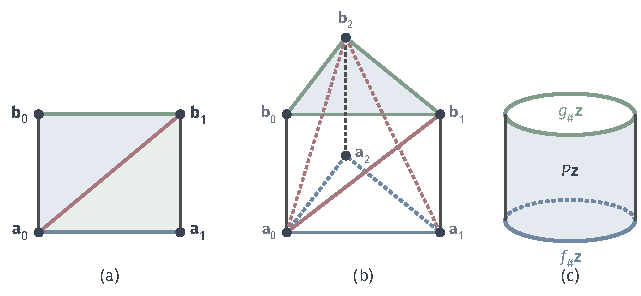
\includegraphics[width=108.511mm]{figures/04-spaces-measures-and-geometry/01-topology-and-metric/tikz/homol-prism/figure.pdf}
  \caption{棱柱的切分与同伦扫出的柱面。(a)$\Delta^1\times[0,1]$被红色对角线切成两个三角形，底边对应$f\circ\sigma$，顶边对应$g\circ\sigma$。(b)$\Delta^2\times[0,1]$被红色线段切成三个四面体$[\bm a_0,\bm b_0,\bm b_1,\bm b_2]$、$[\bm a_0,\bm a_1,\bm b_1,\bm b_2]$、$[\bm a_0,\bm a_1,\bm a_2,\bm b_2]$。(c)闭链$\bm z$被同伦扫成柱面，柱面的边界是顶$g_\#\bm z$减底$f_\#\bm z$。}
  \label{fig:homol-prism}
\end{BookInlineFigure}

要把这个柱面写成奇异链，需要把棱柱$\Delta^k\times[0,1]$切成若干个$(k+1)$维单纯形。记棱柱的底面顶点为$\bm a_i=(\bm e_i,0)$，顶面顶点为$\bm b_i=(\bm e_i,1)$，其中$i=0,\ldots,k$。

对棱柱中的点$\bm u_0,\ldots,\bm u_{k+1}$，记
\[
 \langle\bm u_0,\ldots,\bm u_{k+1}\rangle:\Delta^{k+1}\to\Delta^k\times[0,1]
\]
为把$\bm e_m$送到$\bm u_m$的线性映射，棱柱是凸集，所以它的像在棱柱中。对$X$中的奇异单形$\sigma$，令
\[
 F_\sigma=H\circ(\sigma\times\operatorname{id}_{[0,1]}):\Delta^k\times[0,1]\to Y,
\]
定义\term{棱柱算子}（prism operator）
\begin{equation}
 P\sigma=\sum_{i=0}^k(-1)^i\,F_\sigma\circ\langle\bm a_0,\ldots,\bm a_i,\bm b_i,\ldots,\bm b_k\rangle,
 \label{eq:homol-prism}
\end{equation}
它属于$S_{k+1}(Y)$，并线性延拓为$P:S_k(X)\to S_{k+1}(Y)$。

式中第$i$个单纯形从底面的前$i+1$个顶点出发，在第$i$个顶点处“爬上”顶面，再走完顶面的其余顶点。这$k+1$个单纯形拼成整个棱柱；下面的证明只用到它们的边界之间的相消关系。

\begin{example}[低维的棱柱]
\label{ex:homol-prism-low}
$k=0$时，$\sigma$是一点$x$，$P\sigma$是路径$t\mapsto H(x,t)$，边界为
\[
 \partial P\sigma=g(x)-f(x).
\]

$k=1$时，$\sigma$是路径，正方形$\Delta^1\times[0,1]$被对角线切成两个三角形：
\[
 P\sigma=F_\sigma\circ\langle\bm a_0,\bm b_0,\bm b_1\rangle-F_\sigma\circ\langle\bm a_0,\bm a_1,\bm b_1\rangle.
\]

省略复合号，按式~\eqref{eq:homol-singular-boundary}分别展开两项：
\begin{align*}
 \partial\bigl(F_\sigma\langle\bm a_0,\bm b_0,\bm b_1\rangle\bigr)&=F_\sigma\langle\bm b_0,\bm b_1\rangle-F_\sigma\langle\bm a_0,\bm b_1\rangle+F_\sigma\langle\bm a_0,\bm b_0\rangle,\\
 \partial\bigl(F_\sigma\langle\bm a_0,\bm a_1,\bm b_1\rangle\bigr)&=F_\sigma\langle\bm a_1,\bm b_1\rangle-F_\sigma\langle\bm a_0,\bm b_1\rangle+F_\sigma\langle\bm a_0,\bm a_1\rangle.
\end{align*}

两式相减，对角线$\langle\bm a_0,\bm b_1\rangle$相消，剩下
\[
 \partial P\sigma=F_\sigma\langle\bm b_0,\bm b_1\rangle+F_\sigma\langle\bm a_0,\bm b_0\rangle-F_\sigma\langle\bm a_1,\bm b_1\rangle-F_\sigma\langle\bm a_0,\bm a_1\rangle.
\]

四项依次是$g\circ\sigma$、起点的轨迹、终点的轨迹与$f\circ\sigma$。由于$\partial\sigma=\sigma(\bm e_1)-\sigma(\bm e_0)$，这正是
\[
 \partial P\sigma=g_\#\sigma-f_\#\sigma-P\partial\sigma,
\]
正方形的边界等于顶减底，再减去两条侧边。
\end{example}

例~\ref{ex:homol-prism-low}中的恒等式对一般的$k$也成立，图~\ref{fig:homol-prism}(a)(b)画出了$k=1,2$的切分。

\begin{lemma}[棱柱恒等式]
\label{lem:homol-prism-identity}
对一切$k\geq0$与$\sigma\in S_k(X)$，
\begin{equation}
 \partial P\sigma+P\partial\sigma=g_\#\sigma-f_\#\sigma.
 \label{eq:homol-prism-identity}
\end{equation}
\end{lemma}

\begin{proof}
记$[\cdots]$为$F_\sigma\circ\langle\cdots\rangle$，只需对奇异单形$\sigma$验证。对式~\eqref{eq:homol-prism}的第$i$项取边界，去掉第$j$个顶点：$j\leq i$时去掉的是$\bm a_j$，符号为$(-1)^j$；$j\geq i$时去掉的是$\bm b_j$，它位于第$j+1$个位置，符号为$(-1)^{j+1}$。于是$\partial P\sigma$是下面两组之和：
\begin{gather*}
 \sum_{j\leq i}(-1)^{i+j}[\bm a_0,\ldots,\widehat{\bm a_j},\ldots,\bm a_i,\bm b_i,\ldots,\bm b_k],\\
 \sum_{j\geq i}(-1)^{i+j+1}[\bm a_0,\ldots,\bm a_i,\bm b_i,\ldots,\widehat{\bm b_j},\ldots,\bm b_k].
\end{gather*}

先看$i=j$的项。第一组中$i=j$的项是$[\bm a_0,\ldots,\bm a_{i-1},\bm b_i,\ldots,\bm b_k]$，第二组中下标为$i-1$、去掉$\bm b_{i-1}$的项是它的相反数，因为符号为$(-1)^{2i-1}$。对$i=1,\ldots,k$，二者相消。剩下第一组$i=j=0$与第二组$i=j=k$的项：
\[
 [\bm b_0,\ldots,\bm b_k]=g\circ\sigma,\qquad-[\bm a_0,\ldots,\bm a_k]=-f\circ\sigma.
\]

再看$i\neq j$的项。去掉$\bm a_j$（$j<i$）或$\bm b_j$（$j>i$）后，剩下的单纯形恰好是第$j$个面$\sigma\circ\delta_j$所对应棱柱中的一块：前者是第$i-1$块，后者是第$i$块。这是因为$\delta_j\times\operatorname{id}$把较小棱柱的顶点按次序线性地送到这些顶点上，并满足
\[
 F_\sigma\circ(\delta_j\times\operatorname{id})=F_{\sigma\circ\delta_j}.
\]

按定义展开
\[
 P\partial\sigma=\sum_j(-1)^jP(\sigma\circ\delta_j)
 =\sum_{i>j}(-1)^{i+j-1}[\cdots\widehat{\bm a_j}\cdots]+\sum_{i<j}(-1)^{i+j}[\cdots\widehat{\bm b_j}\cdots],
\]
它恰好是$\partial P\sigma$中$i\neq j$各项的相反数。三部分相加，即得式~\eqref{eq:homol-prism-identity}。
\end{proof}

式~\eqref{eq:homol-prism-identity}的几何含义是：柱面的边界等于顶减底，再减去边界扫出的侧面。这是例~\ref{ex:homol-prism-low}中“正方形的边界”在一般维数上的写法。

\begin{theorem}[同伦不变性]
\label{thm:homol-homotopy-invariance}
若连续映射$f,g:X\to Y$同伦，则
\begin{equation}
 f_*=g_*:H_k(X)\to H_k(Y)
 \label{eq:homol-homotopy-invariance}
\end{equation}
对一切$k$成立。因此，若$f:X\to Y$是同伦等价，则$f_*$是同构；同伦等价的空间有同构的奇异同调。
\end{theorem}

\begin{proof}
对闭链$\bm z$，由引理~\ref{lem:homol-prism-identity}，
\[
 g_\#\bm z-f_\#\bm z=\partial P\bm z+P\partial\bm z=\partial P\bm z,
\]
右端是边界链，所以$g_*[\bm z]=f_*[\bm z]$。

若$h$是$f$的同伦逆，由定理~\ref{thm:homol-induced-map}与刚才的结论，
\[
 h_*f_*=(h\circ f)_*=(\operatorname{id}_X)_*=\operatorname{id},
\]
同理$f_*h_*=\operatorname{id}$，所以$f_*$是同构。
\end{proof}

这个结论称为同调的\term{同伦不变性}（homotopy invariance）。它在第~\ref{sec:homol-homotopy}节与本节之间架起桥梁：同伦等价保留的代数信息，至少包括全部Betti数。

\paragraph{单点与可缩空间}
单点空间$\{p\}$在每个维数恰有一个奇异单形$\sigma_k$（常值映射），并且$\sigma_k\circ\delta_i=\sigma_{k-1}$。由式~\eqref{eq:homol-singular-boundary}，
\[
 \partial_k\sigma_k=\sum_{i=0}^k(-1)^i\sigma_{k-1}=
 \begin{cases}0,&k\text{为奇数},\\ \sigma_{k-1},&k\geq2\text{为偶数}.\end{cases}
\]

所以$\partial_1=0$，$\partial_2$是同构，$\partial_3=0$，$\partial_4$是同构，依此类推。$k$为奇数时$\ker\partial_k=S_k$被$\operatorname{im}\partial_{k+1}$占满；$k\geq2$为偶数时$\ker\partial_k=0$。于是
\[
 H_0(\{p\})\cong\mathbb R,\qquad H_k(\{p\})=0\ (k\geq1).
\]
由定理~\ref{thm:homol-homotopy-invariance}，可缩空间（如区间、圆盘、$\mathbb R^n$）的同调与单点相同。

\paragraph{环带与圆周}
回到本章开头的问题。由例~\ref{ex:homol-annulus-retraction}与定理~\ref{thm:homol-retract-equivalence}，包含映射$i:S^1\to A$是同伦等价。由定理~\ref{thm:homol-homotopy-invariance}，$i_*$是同构，所以
\[
 H_1(A)\cong H_1(S^1)\cong\mathbb R.
\]
更具体地，环绕圆周一周的一维闭链，在环带中仍是不能填掉的闭链；环带比圆周多出的“厚度”被形变收缩压平，不产生新的同调类。

由此兑现第~\ref{sec:homol-homotopy-equivalence}小节的承诺：$H_1(A)\neq0=H_1(\{p\})$，所以环带不可缩。

同一论证还说明圆盘不能回缩到边界圆周上。若$r:D^2\to S^1$是回缩，$j:S^1\to D^2$为包含，则$r\circ j=\operatorname{id}_{S^1}$，于是$r_*\circ j_*$是$H_1(S^1)\cong\mathbb R$上的恒等映射。可是$j_*$经过$H_1(D^2)=0$，复合只能为零，矛盾。

\paragraph{同调不能判定什么}
同伦不变性同时划出了同调的边界。圆盘与单点同伦等价，同调相同，却不同胚；所以同调相同不能推出同胚，这一点在第~\ref{sec:homol-homology-spaces}小节已经用复形看到。

同调相同也不能推出同伦等价。环面与“两个圆周和一个球面粘在一点”的空间，Betti数都是$(1,2,1)$，却不同伦等价；区分它们要用基本群或同调环等更细的工具，证明需要另外建立这些工具。同调是检验“不同”的工具：Betti数不同，就足以断定两个空间既不同胚，也不同伦等价。
